% Modelling infectious disease dynamics towards informed public-health interventions, with application on \textsc{covid}-19 and cholera.
\chapter*{Introduction} % broad introductio
\addcontentsline{toc}{chapter}{Introduction}
\markboth{Introduction}{}
%epidemics as phenomena
 %d  unevenly distributed among populations. 
 % improverished communties around the world. %public health issue in many countries, and it's elimination of Global North countries -- . 
 %\section{Context}
 Centuries after the first cholera pandemics and 160 years after the realisation that safe drinking-water, adequate sanitation and hygiene prevent its transmission, cholera remains a threat to millions living in hotspots or at risk areas. The recent emergence of the new coronavirus disease 2019, \textsc{covid}-19, and the strain it put on even world's most advanced healthcare systems recalls the constant risks posed by emerging diseases. 
While elimination might be involved, public-health policies have proven the effectiveness of interventions against infectious diseases, showing that deaths are preventable. The control of infectious diseases presents challenges accross every dimensions of environmental and human health; in order to prevent spillover events, to block transmission routes, and to protect and treat every person adequately and equally. 

In the fight against infectious diseases, a serie of successes -- attributable to \eg hygiene, vaccines, antibiotics, safe water, ... -- brough the hope of a global and durable reduction of the burden, and a road towards elimination for many diseases. Especially in privileged communities, long-term improvements have been achieved for many of the diseases that have shape the history of humanity. While these progresses show that infectious diseases are not a necessary fate, setbacks on the control of existing and emerging pathogens remind us the ongoing threat they poses on public-health. Indeed, the current global health picture is marked by inequalities in the distribution of the burden, which disproportionaly piles up on already impoverished communities, in conflict zone or after natural disasters. To date, communicable diseases cause approx. 15\% of global deaths every year\cite[-4\baselineskip][Table 1, excl. non-transmissible neonatal and maternal diseases and nutritional diseases; pre-\textsc{covid}-19 estimates]{Roth:GlobalRegionalNational:2018}, and nearly 1/3 of all child deaths are caused by pneumonia and diarrhoea alone\cite[][\ie 2\textsc{M} deaths among under 5, every year.]{WHO:EndingPreventableChild:2013}.
 
Epidemics -- the rapid spread of an infectious diseases in a population -- are a complex phenomenas, the results of interactions between pathogens, enviroment, societies and individuals\cite{Rinaldo:RiverNetworksEcological:2020a, Buckee:ThinkingClearlySocial:2021, Heesterbeek:ModelingInfectiousDisease:2015}. Public-health policies strive to save lives by designing effective mitigitation measures. Among the many aspects of designing such policies, the difficulties of reasoning on uncertainties araising from complex multi-factorial interactions with scarsed and biased information and understanding limit the possibilites. 

Models -- conceptuals representations of systems -- are tools to reason about the world. Historically, conceptuals models of the propagation of diseases, from divine retribution to miasma theory, has motivated more (quarantine) or less (persecution) effective approaches to the control of these pests. Scientific breaktrough in biology and medicine, with the identifications of pathogens and their transmission route, opened the path for improved prevention and treatments. Novel statistical modeling approaches\cite[-3\baselineskip]{Freedman:AssociationCausationRemarks:1999} developed in the 20th century -- and continously improved ever since\cite{Gelman:WhatAreMost:2021} --  provided a formal framework to reasons about the propagation of a disease in a population. It allows to deal with bias on data collection, to account for epistemic uncertainties, and to encompass uncertainties in the transmission dynamics, the affected populations and the effect of intervention policies in a principled way. The toolbox was further re-enforced by breakthrough advances in mechanistic modeling applied to disease transmission, starting from SIR compartmental models\cite{Kermack:ContributionMathematicalTheory:1927, Anderson:PopulationBiologyInfectious:1979}, which divide the population depending on their status with respect to the disease. Later, advances in computing power proved a paradigm shift in dealing with the available evidence, and in representing and infering features. 

The present thesis explore compartmental models as ways to reason about infectious disease transmission, and as tools to guide decisions. It aim at answering a series of research questions, each question being a variations of: why do things spread the way they do ? and how can it be prevented from spreading ? It answers these questions using extensively computer-age modeling and inference methods, in a cyclical process represented in fig.~\ref{fig:modeling}. %cyclical pricess cycle: model design, inference, evaluation, results, communication, listening and an important feedback loop.

\begin{figure*}\centering
  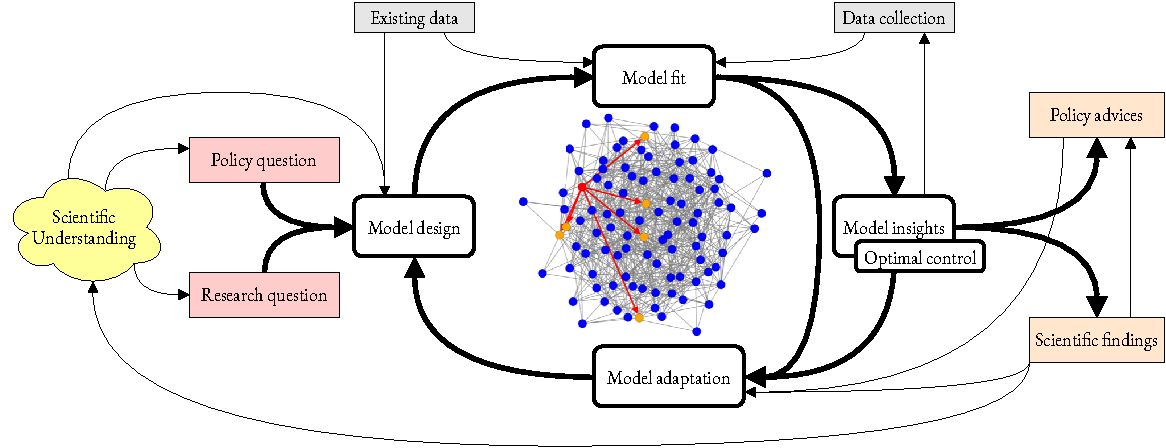
\includegraphics{fig/modeling_cycle_new}
  \caption[Process for infectious disease modeling][-1\baselineskip]{Process for building models of infectious diseases, with important feedback loop on model results. Appart from data collection, all boxes were explored in the present thesis. The central figure of an agent-based model of disease transmission in a random graph was made by Thomas Fry,  master student supervised during this thesis (with permission).}\label{fig:modeling}
\end{figure*}

Despite its recent formalism, statistical inference remains an art, uncomfortably dependent on the practitioners and their backgrounds\sidenote[][8\baselineskip]{Multimodeling studies and collaborative experiments strive to mitigate this issue by bringing together assumption and projections by different groups. See \eg \url{covid19forecasthub.org/community}}. While designing models, choices on what to include and how to express the supposed dynamics depends on the underlying knowledge of the processes and the available data. 

Once a model has been built, statistical inference conditions the model on the observed data. It allows to infer unobserved quantities from reported ones, such a lockdown intervention from hospitalization and deaths. After an evaluation of the \textit{fit} of the model and the implication on the results, if the predictive accuracy is satisfying, comes the time to answer the research questions. The model many be used to identify transmission routes, as a reproduction of reality. Another way to use a model that reproduce observed dynamics may be as substitute for experiments, to simulate scenarios and to evaluate the impact of hypothetical polices on a virtual system. It determines the range of expectations one may expect with regard to real world consequences of tested policies. Communication of modeling results, with proper awareness of limitation and scope finally provide the opportunity for feedback and eventual adaptation of the model\cite{Heesterbeek:ModelingInfectiousDisease:2015}.

Another use of modeling presented in this thesis is the application of optimal control to interventions against infectious diseases. Optimal control are novel methods, mostly used in automative engineering, that enable the automatical design of planning interventions. While technicals adaptations are necessary to allow its use on epidemics, this rigorous framework identifies the most effective control measures under a set of operational constraints, discovering invisible features and policies. These optimal interventions exploit every features of the complex interactions modelled, allowing to \eg best allocate a limited vaccine supply in space. Such tools, at their infancy and requiring accurate models, are promising as reasoning aid, uncovering another facet of disease transmission, and for effective control of an epidemics.
\begin{table*}[t]
\label{tab:allmodels}
\centering\small
\begin{tabularx}{\textwidth}{x{14mm}cccx{15mm}cx{15mm}p{30mm}}
\toprule
   \small{\textsc{Chapter}}     & Disease           & Comparments & Processes         & \small{$N_{\text{spatial}}$} & Fit       & Aim            & Reference\\
\midrule
4 & Cholera           & SEIR+B      & Stochastic    & --           & MIF like  & explain         & \tiny{\fullcite{Lemaitre:RainfallDriverEpidemic:2019}}\\
4 & Cholera           & SEIR+B      & Deterministic & --             & MCMC-like & explain        & \tiny{\fullcite{Lemaitre:RainfallDriverEpidemic:2019}}\\
5  & Cholera           & SEAIR$^3$+V & Stochastic    & 10        & MIFlike   & project (scenarios)       & \tiny{\fullcite{Lee:AchievingCoordinatedNational:2020}} \\ \addlinespace
6  & \textsc{\textsc{covid}}-19 & SEI$^3$R+VH & Stochastic    & 3’000+    & MCMC-like & project (scenarios)        & \tiny{\fullcite{Lemaitre:ScenarioModelingPipeline:2021}} \\
7  & \textsc{\textsc{covid}}-19  & SEI$^3$R+H  & Stochastic    & --             & MIF-like  & infer           & \tiny{\fullcite{Lemaitre:AssessingImpactNonpharmaceutical:2020}}\\
8  & \textsc{\textsc{covid}}-19  & SEIAR+VH    & Deterministic & 107       & MCMC-like & optimal\newline control & \tiny{\fullcite{Lemaitre:OptimizingSpatiotemporalAllocation:2021}}\\ 
\bottomrule
\end{tabularx}
\caption[Presentation of the models described in this thesis]{Presentation of all  compartmental models described in this thesis. In columns Compartments, in addition to susceptible S, exposed (incubating) E , infected (infectious, symptoms) I, infected (infectious, no symptoms) A and recoved R, it is indicated by H that additional compartments to represent the healthcare facilities (hospitalisation, ICUs), by V compartments for vaccinationated, and by B the dynamical modeling of an environmental reservoir. The exponent denotes the multiplication of the same compartment to change the residence distribtuion, using the linear-chain trick. Two fitting procedure are used: frequentist iterated filtering and bayesian Markov-Chain-Monte-Carlo.}
\end{table*}
%\section{Aim and outline}
The present thesis has been developed within the Swiss National Foundation project ``Optimal control of intervention strategies for waterborne disease epidemics (\textsc{snf} 200021–172578)’’. It initial goal was to develop a decision support system for the real-time design of optimal intervention strategies against cholera, which includes an operational forecasting tool coupled with an optimal control solver. This framework has been developed, albeit for \textsc{covid}-19 transmission in Italy, and is presented in \textsc{Chapter 8}. Indeed the \textsc{covid}-19 pandemic has disrupted the research plan of the present thesis. As a consequence, it happens to associate two antipodean diseases. Cholera, one of the most ancient recorded disease\footnote[][10\baselineskip]{History of pre-pandemic cholera is uncertain but numerous accounts of the disease are supposed from as early as 400\textsc{bce}. See \fullcite[p. 95]{Byrne:EncyclopediaPestilencePandemics:2008}.}, has caused 7 pandemics in the modern era. In contrast, \textsc{covid}-19 earliest known onset of symptoms is on December 1, 2019. The pathogen for cholera is a bacteria, \textit{Vibrio Cholerae}, responsible for heavy watery diarrhea, whereas \textsc{SARS-CoV-2}, \textsc{covid}-19’s pathogen, is a virus responsible for respiratory infections. Cholera belongs to the negletected tropical diseases, a class of understudied infections while the \textsc{covid}-19 pandemic as sparked an unprecented accumulation of evidence\sidenote[][]{With more than 190'000 peer-reviewed papers and many more preprints, website and reports published at the time of writing. Estimation from: \fullcite{COVID-19OpenAccessProject:LivingEvidenceCOVID19:2020}}. Differs also the posited transmission route (fecal-oral vs. respiratory route), the affected communities (``poorest of the poor”, higher severity on children vs. global, higher severity on elders), etc... Despite these differences, Cholera and \textsc{covid}-19 shares mechanisms that makes their transmission sustainable in populations and causes pandemics, a regretully high tool on humanity, and repartition of burden that echoes inequal access to care and disproportionately affecting stigmatized commuties. Both cholera and \textsc{covid} are infectious diseases -- with the potential of starting epidemics and pandemics, and the scientific methods to answer questions about the spread and control is has some similarities between these diseases and others.


A set of 5 models, see tab. \ref{tab:allmodels}, is proposed in this thesis, with features that depends on the disease, the context, the possible control measures and the quantity of uncertaintainties associated with the data and the processes. Some models have stochastic transitions, other are mostly deterministic, some model human mobility accross regions whereas others assumes well-mixed population. Despite the foregoing differences, all the models presented in this thesis are compartmental with some mechanistic components; all are based on the SIR model.

The work presented extensively builds on the ECHO laboratory expertise on the spatially-explicit modeling of cholera transmission\footnote{and waterborne diseases in general; see: \fullcite{Rinaldo:RiverNetworksEcological:2020a, Rinaldo:Reassessment20102011:2012}}. The group has developed over a decade a rainfall-mediated, spatially explicit cholera model that has inspired each of the other models presented in this thesis. The original,  model developed in the group, is presented in \textsc{Chapter 3}, with a short introduction on the ancient disease that is cholera, with a rich and sorrowful history.

Cholera is the focus of two additional chapters. The explanatory power of two influential models of cholera transmission and its link to rainfall are compared in \textsc{Chapter 4}, on an outbreak inJuba, South-Sudan. In \textsc{Chapter 5}, a scenario planning estimation of the probability of eliminating cholera from Haiti with a mass vaccination campaign is presented; this work has been carried within the framework of a multi-modeling study with other groups, and input from the ministry of health of Haiti.
\marginnote[-5\baselineskip]{Most bibliographic items and some additional precision are presented as margin notes for convenience. However, the full bibliography is included at the end of the thesis.}
The remaining chapters focuse on \textsc{covid}-19. In \textsc{Chapter 6} some facets of dealing with uncertainties from the early days of the pandemic are uncovered, with a focus on a pipeline for scenario modeling that has been used to inform gouvernements, in the United- States and other countries. 
An inference study to estimate the impact of the interventions against \textsc{covid}-19 in Switzerland is presented in \textsc{Chapter 7}.
%\marginnote[-5\baselineskip]{Incidentaly, this organisation reflects the chronogical order of the work.}
Finally, a tentative to connect an optimal control framework to an epidemiological model towards the allocation of \textsc{covid}-19 vaccines in Italy is presented in \textsc{Chapter 8}.

